\documentclass[sigconf]{acmart}

\usepackage{booktabs} % For formal tables


% Copyright
%\setcopyright{none}
%\setcopyright{acmcopyright}
%\setcopyright{acmlicensed}
\setcopyright{rightsretained}
%\setcopyright{usgov}
%\setcopyright{usgovmixed}
%\setcopyright{cagov}
%\setcopyright{cagovmixed}


% DOI
\acmDOI{10.475/123_4}

% ISBN
\acmISBN{123-4567-24-567/08/06}

%Conference
\acmConference[GECCO '17]{the Genetic and Evolutionary Computation Conference 2017}{July 15--19, 2017}{Berlin, Germany}
\acmYear{2017}
\copyrightyear{2017}

\acmPrice{15.00}


\begin{document}
\title{Modeling Human Interactions in Collaborative Interactive 
 Evolutionary Computation}
%\titlenote{Produces the permission block, and
%  copyright information}
\subtitle{Anonymized Version}
%\subtitlenote{The full version of the author's guide is available as
%  \texttt{acmart.pdf} document}


\author{Ben Trovato}
\authornote{Dr.~Trovato insisted his name be first.}
\orcid{1234-5678-9012}
\affiliation{%
  \institution{Institute for Clarity in Documentation}
  \streetaddress{P.O. Box 1212}
  \city{Dublin} 
  \state{Ohio} 
  \postcode{43017-6221}
}
\email{trovato@corporation.com}

\author{G.K.M. Tobin}
\authornote{The secretary disavows any knowledge of this author's actions.}
\affiliation{%
  \institution{Institute for Clarity in Documentation}
  \streetaddress{P.O. Box 1212}
  \city{Dublin} 
  \state{Ohio} 
  \postcode{43017-6221}
}
\email{webmaster@marysville-ohio.com}

\author{Lars Th{\o}rv{\"a}ld}
\authornote{This author is the
  one who did all the really hard work.}
\affiliation{%
  \institution{The Th{\o}rv{\"a}ld Group}
  \streetaddress{1 Th{\o}rv{\"a}ld Circle}
  \city{Hekla} 
  \country{Iceland}}
\email{larst@affiliation.org}

\author{Lawrence P. Leipuner}
\affiliation{
  \institution{Brookhaven Laboratories}
  \streetaddress{P.O. Box 5000}}
\email{lleipuner@researchlabs.org}



\begin{abstract}
The necessary intervention of humans in interactive evolutionary
computational systems has inherent drawbacks arising from the very nature of 
the algorithms, namely, the human fatigue caused by the interaction, and
the boredom arising when users evaluate a large number of artifacts 
many of which are not interesting or are very similar to each other.
To tackle these issues, in this paper we
propose a human-centered framework to model 
the complex interactions on these system.
Three case studies are presented where the model is applied in the 
development of evolutionary interactive systems, with different techniques:
volunteer-collaborative, unplugged and sensor-based. 
Both conceptual and implementation details are provided where the   
technique is applied to measure and increase user engagement and participation.
Our experiments show that the model can be successfully applied in a
gamification technique developed to increase user engagement, which
implies that this technique can successfully be used to 
decrease user fatigue and thus increase {\em performance} of the
interactive system.
\end{abstract}

%
% The code below should be generated by the tool at
% http://dl.acm.org/ccs.cfm
% Please copy and paste the code instead of the example below. 
%
\begin{CCSXML}
<ccs2012>
<concept>
<concept_id>10003120.10003130.10003233</concept_id>
<concept_desc>Human-centered computing~Collaborative and social computing systems and tools</concept_desc>
<concept_significance>500</concept_significance>
</concept>
<concept>
<concept_id>10010147.10010178.10010205.10010206</concept_id>
<concept_desc>Computing methodologies~Heuristic function construction</concept_desc>
<concept_significance>300</concept_significance>
</concept>
<concept>
<concept_id>10010147.10010178.10010205.10010207</concept_id>
<concept_desc>Computing methodologies~Bio Inspired Algorithms</concept_desc>
<concept_significance>300</concept_significance>
</concept>
<concept>
<concept_id>10010147.10010919.10010172</concept_id>
<concept_desc>Computing methodologies~Distributed algorithms</concept_desc>
<concept_significance>300</concept_significance>
</concept>
</ccs2012>
\end{CCSXML}

\ccsdesc[500]{Human-centered computing~Collaborative and social computing systems and tools}
\ccsdesc[300]{Computing methodologies~Heuristic function construction}
\ccsdesc[300]{Computing methodologies~Distributed algorithms}
% We no longer use \terms command
%\terms{Theory}

\keywords{Interactive evolutionary computation, Human Centered Computing}


\maketitle

\section{Introduction}
% Main Ideas:

% IEAs
% Human Based Computation
% C-IEAs
% Problems
% Volunteers 
% Human Centered
% C-IEA Complex Interactions
  % User -> Human
  % Social Network
  % Devices IoT
  % Activities
  % Engagement

% Why an HC Framework (Objectives)  
% Presentation 


% IEAs
Interactive evolutionary computation (IEC) systems are, in general, evolutionary methods
whose fitness evaluations are performed by humans through an interactive 
system \cite{eiben2015interactive}.
They are usually applied in problems where the fitness function is not known or simply
does not exist, and the result of optimization should fit a certain human need or desire. 
That is why their use-case includes the evolution of objects with subjective characteristics
such visual appeal or attractiveness \cite{biomorphs} as well as others where human behavior is 
considered, for instance the optimization of teamwork \cite{kosorukoff2002evolutionary}
or creativity \cite{yu2011cooks}.
% Human Based Computation
These IEC systems are an interesting venue of research, since they have demonstrated 
their ability for effectively 
producing art and design \cite{Bentley:1999:intro,Sims:1991,todd:1992,evoeco},
as well as other artifacts in many other domains \cite{ie1}. In those cases when 
human interaction is responsible of other 
aspects of the evolutionary process, some authors classify these IEC methods 
as human-based evolutionary computation \cite{kosorukoff2001human} 
or as human-based computation \cite{quinn2011human}.
% Problems
However, the necessary intervention of humans, brings certain challenges 
to designers of IEC methods namely, human evaluations are slow and expensive, there is
human fatigue caused by the interaction \cite{ie1}, and also boredom arise
when users evaluate a large number of phenotypes, 
many of which are not interesting or are very similar to each other.
% C-IEAs
Moreover, the performance of these systems effectively depends on the number of users
they are able to include; to reach more users,
IEC systems are some times developed as web applications depending on web visitors to help
with the search, using both anonymous and registered users. Some systems 
employ a collaborative technique, where several users participate in 
the evaluation, this method is called Collaborative-IEC (C-IEC)
\cite{picbreeder,seyama2016development,wagy2014collective}.
% Volunteers 
Having a volunteer system can lower the requirements for anyone to participate in
the experiment thus increasing the {\em performance} of the whole system. But using a volunteer based 
system raises other issues \cite{sarmenta2001volunteer,web:BOINC}, such as the 
volunteer\'s lack of accountability, and the need to build trust between participants and project
owners. Other issues for project owners are also the difficulty of establishing 
the amount of time and resources a volunteer is willing to spend on the system, 
and how they decide if they participate or not \cite{JJ:2016}. 

% Human Centered
In order to increase volunteer participation and to tackle some of the issues mentioned above,  
we proposed a software framework following a human centered design \cite{greenhouse2012human},
giving extensive attention to volunteers, not only because their
explicit evaluation is essential, but also because the context of the 
interaction affects the system as a whole.

For example, in a C-IEC application fitness assignment depends on the
actions of a social network of users.  These actions are triggered when 
they tag, share, rate, store or delete a phenotype. 
Then, the selection of parents could depend on the previous actions, leveraging information, 
such as the fact that they both have the same tag, or were shared by
similar users.

Data available from the interaction is also used to increase the engegment of 
users in the system by applying  gamification techniques. Gamification is defined by 
Deterding et al. \cite{deterding2011game} as
\begin{quote}
  the use of game design elements in non-game contexts.
\end{quote}  
The gamification element employed in this case study has been a rewarding mechanism  
\cite{dubois2013understanding}. In general rewards  consist of a reputation system 
with score points, levels and leader boards. Points are awarded to users in response of 
the accomplishment of certain activities that need to be encouraged. Levels depend
on the score and certain features of the game are only available to gamers when 
they reach a giving level. % Say what we are doing in this case - JJ
%%%
%%% Change if case studies change
%In this work, a case study consisting in a web application for evolving artistic drawings
%is presented, providing both conceptual and implementation details of the framework. 
%In order to test the framework three versions of the application are compared to
%measure the degree of relationship between users and their participation,
%when appling a gamification technique. 
In this work, three case studies are presented. First, the development of a web based C-IEC application 
for evolving artistic drawings is described, to give the reader details about 
the utilization of the proposed framework. Then, a rewarding mechanism is 
implemented in the same application, to study the changes in participation,
when appling a gamification technique. Later two other case studies are briefly presented
to show how the framework is applied in other domains.

The rest of this paper is organized as follows.
Section \ref{sec:related} presents related work on the topic 
of Interactive Evolution. Then, Section \ref{sec:framework} presents the human centered framework of
for C-IEC appliactions which the main proposal of this work. Next three case studies are presented in
sections 

An implementation using the ES-I framework 
is detailed in Section \ref{sec:implementation}.
The case study and results are presented in Sections \ref{sec:experiments} and  
\ref{sec:results}. Finally, a concluding remarks are provided in Section \ref{sec:conclusions}.

\section{Related Work}
\label{sec:related}

An early example of web based collaboration is the work by 
Langdon \cite{langdon:2004}, which evolved fractal representations of virtual creatures. 
Similarly, Secretan et al. \cite{picbreeder} and Clune and Lipson \cite{forms} 
use web-based IEAs to evolve artistic artifacts using a generative encoding.
Another example is the Galapagos Project \cite{sims1997interactivity},
an exhibit in the Tokyo Multimedia Museum (1997--2000) 
were visitors interacted with images presented in 
twelve displays by selecting those they found most aesthetically interesting by standing on
step sensors in front of them, presenting an example of a non web C-IEC system. 

Some C-IEC systems promote user engagement by presenting interesting information to 
users, for instance the genetic lineage of each phenotype or the most popular or 
best rated solucion\cite{picbreeder,forms}.In a recent work by 
Wagy \& Bongard \cite{wagy2014collective} user interaction 
is needed for evaluating the fitness and developing
new designs of robot locomotion. Collaboration is encouraged by gamifying the system 
using the maximum distance indicator to inspire the user to try and ``beat'' previous designs. 
In any case, using gamification techniques imply that we must deal with interactive evolutionary
system as socio-technical constructs, where the social aspects are
essential to understand its dynamics. In this sense, conclusions
reached with other systems such as NodEO \cite{DBLP:conf/gecco/MereloCGCRV16}
can also be applied to this system; and applying social 
network techniques such as graph analysis
to their study will allow us to understand them more thoroughly. 
% C-IEAS
Given the human fatigue limitation when applying IEAs, some authors 
have tried to mitigate the problem by allowing the algorithm to 
collaborate with the user, so that sometimes 
users perform the evaluation,  but also specific measures are included 
into the algorithm to perform the
evaluation of some features automatically. For instance, 
Reis et al. added some terrain measures (such as accessibility and edge length) 
to a standard  IEC in \cite{DBLP:journals/soco/FradeVC12}. 
This way the algorithm was capable of providing  terrains that would otherwise have needed
users evaluation for these specific features. Seyama and Munetomo \cite{seyama2016development}
also propose the reduction of the user fatigue by using 
a collaborative filtering algorithm to show only the information utilized by similar users as 
they collaborate with a large number of users for the interactive modeling of 3D glasses. 
The framework and data model for 
representing the interactive process of C-IEC systems is proposed next
% Volunteer Based
% HBC
% Engagement Techniques
% Models

\begin{figure*}[!t]
    \centering
        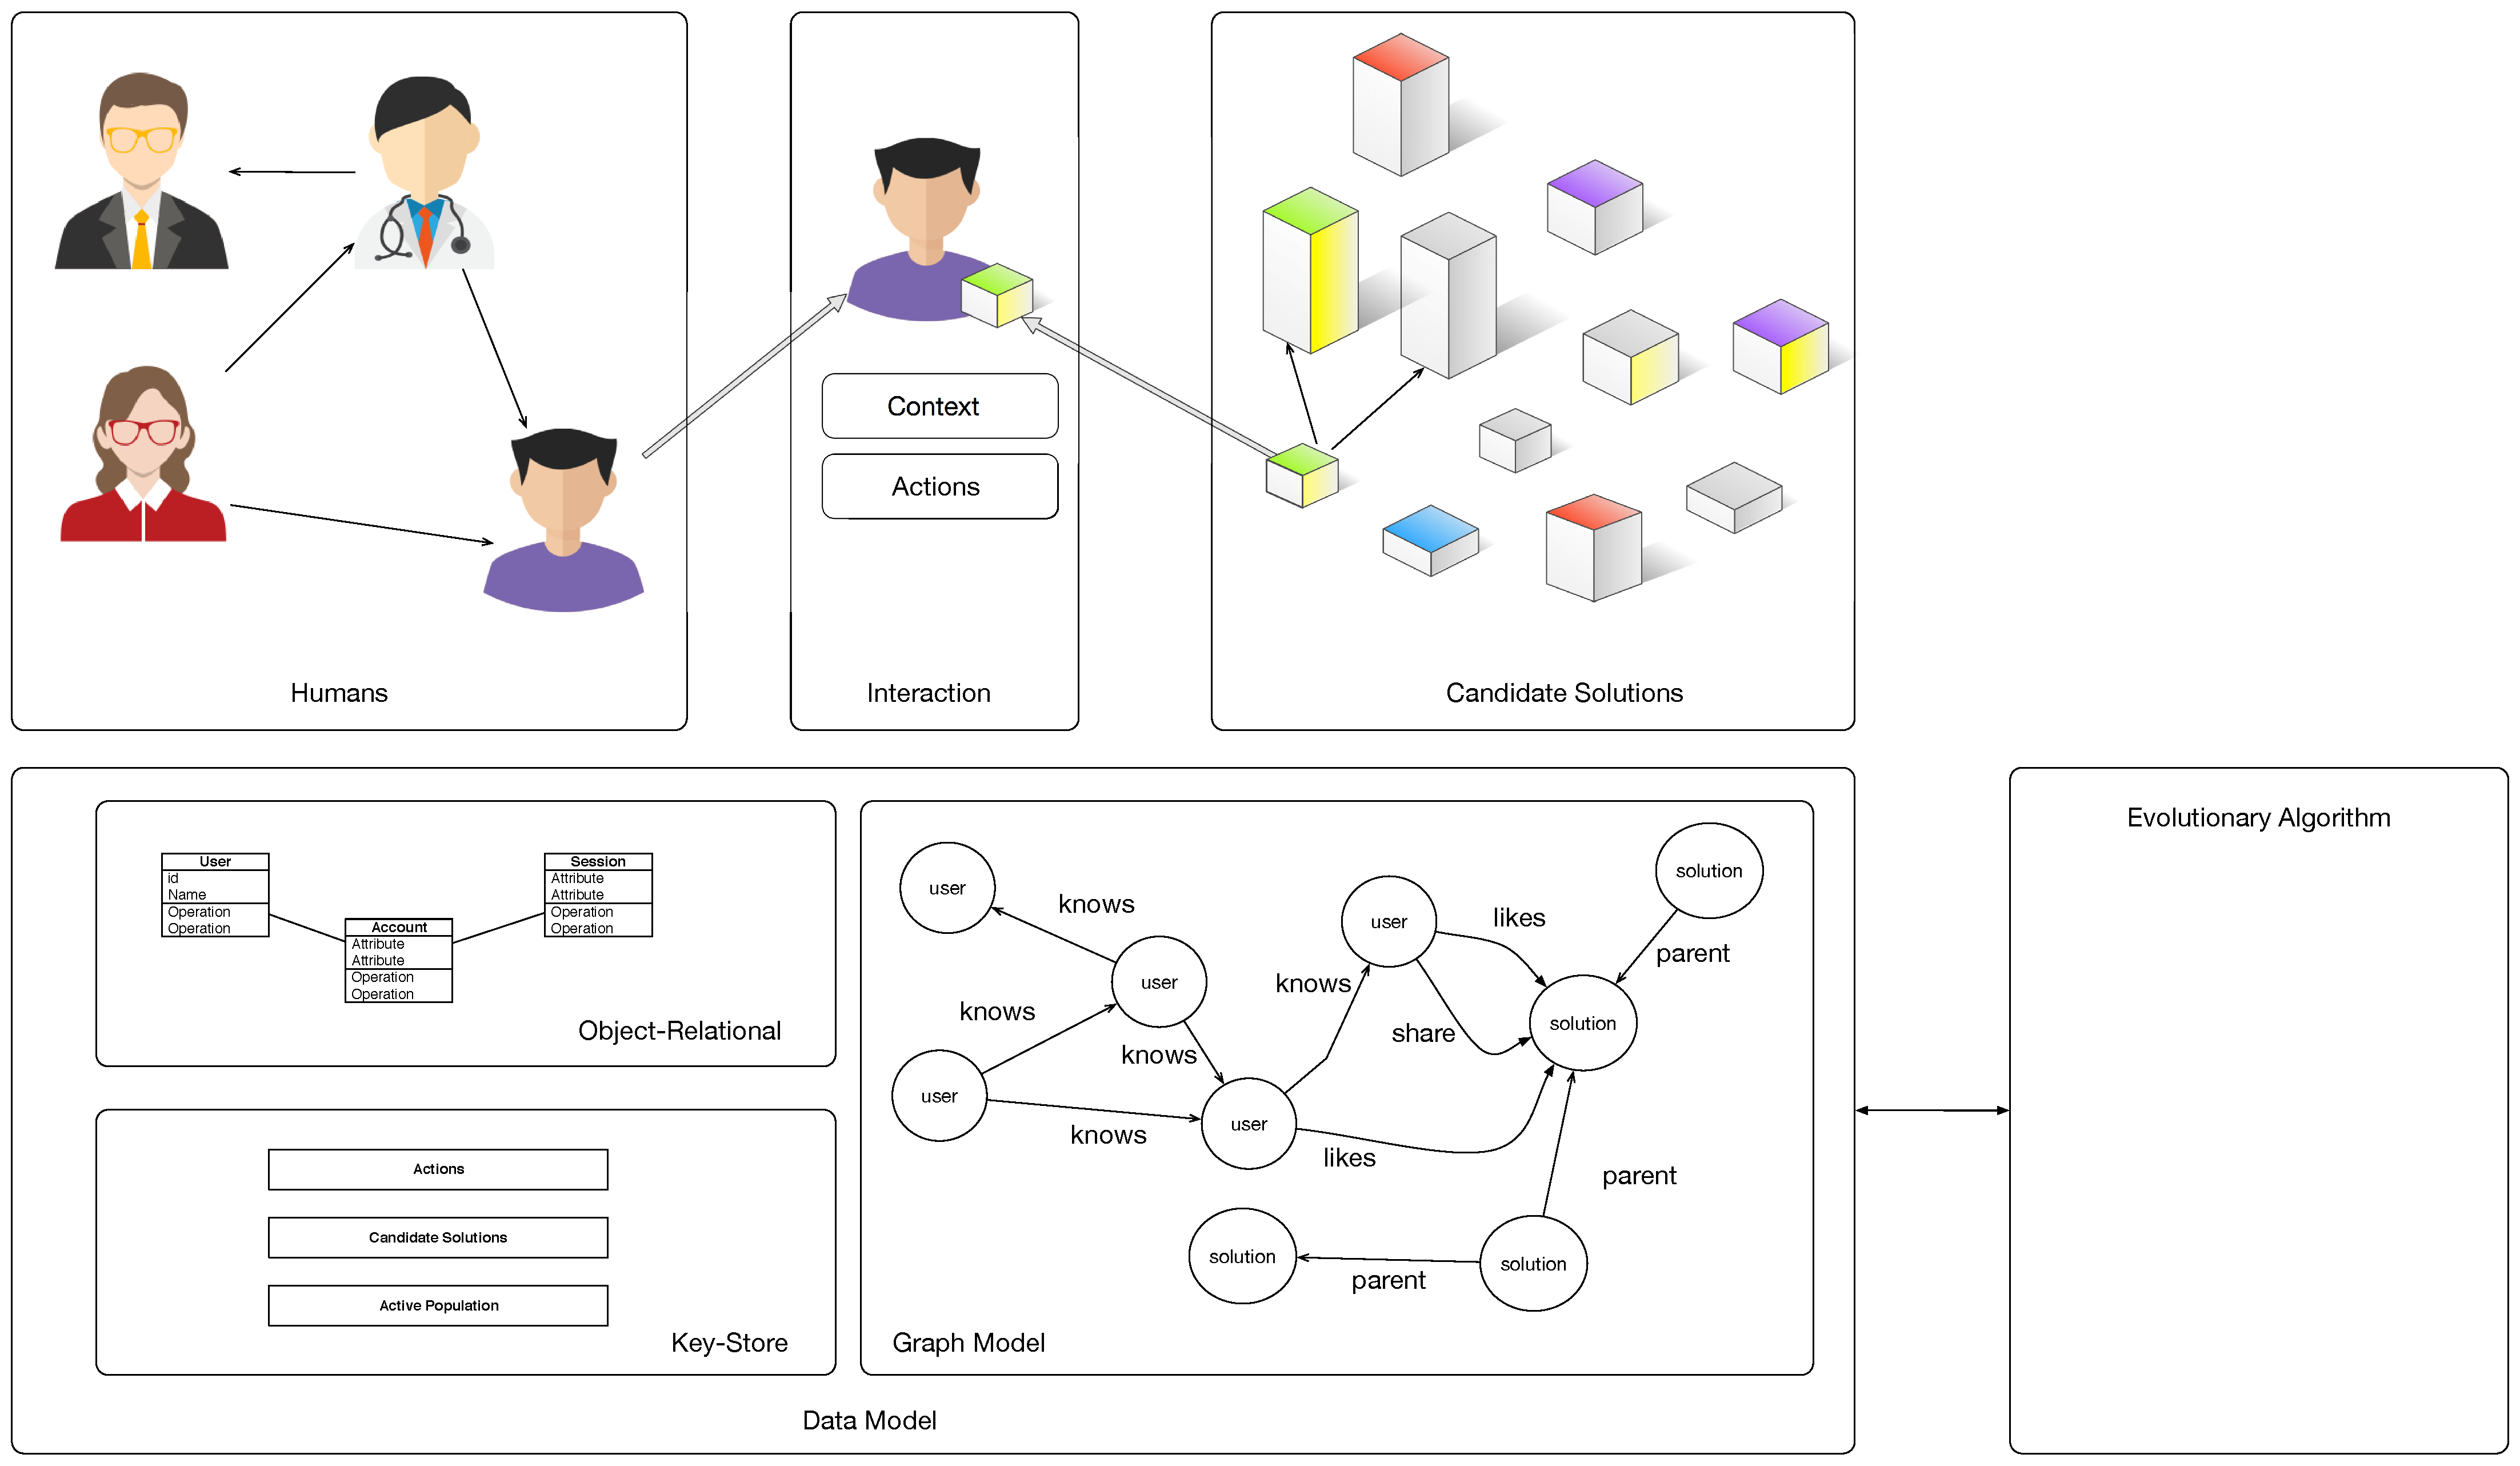
\includegraphics[width=5.5in]{img/framework.eps}
    \caption{IEC Human-centered framework.}
    \label{fig:hc_framework}
\end{figure*}

\section{Human-Centered IEC Framework}
\label{sec:framework}
The general goal of this line of research is to develop a human-centered \cite{gasson2003human} 
software framework for interactive evolutionary computation (IEC). 
A framework is defined as a reusable architectural design together
with an implementation \cite{campbell1991choices}, in this case 
providing generalized components to developers of IEC systems. 

The proposed framework includes components that can be refined to increase
participation and also to minimize the amount of evaluations needed for the evolutionary 
process in a given IEC application. Software frameworks often have a vison or a way 
of thinking \cite{carneiro2010introducing} guiding their
design. Before diving into details the main design considerations of the
framework are explained next: 

\begin{itemize}
\item {\bf Users are human} 
  The framework follows the approach of human centered computing \cite{sebe2010human},
  in which the context, environment, interfaces, preferences, accessibility, human relations,
  cognitive limitations, culture, creativity and other human aspects are an integral part 
  of the system. Humans are the computing resorces of the system, having unique characteristics
  as those identified by Sun \& Dance \cite{Sun2013}
\begin{quote}
  (1) humans can solve computer hard problems; (2) humans are very good at exception handling,
  (3) humans have creativity, (4) humans have cognitive load limitation, (5) humans are
  vulnerable to psychological manipulation, (6) humans are prone to errors,
  especially for reflective tasks.
\end{quote}  


\item {\bf Users are volunteers} Users donate their computing resources, so they are 
unaccountable, some times they try to game the system. Project owners must actively promote and
design the interactive system to engage volunteers \cite{oh2015clicking}. % Define
\item {\bf Users are not alone}
  Relationship between users in an interactive evolutionary algorithm can be modeled
  as a social network, with well established semantics, algorithms and metrics 
  \cite{ahuja1993network}.
  A graph model could enable researchers to find other ways of identifying leaders of 
  opinion or measuring the similarity between user's preferences. 
  These measures can then be used by recommender algorithms selecting 
  phenotypes according users' preferences. 

\item {\bf Context of use matters}
  \textit{Context} In computer science Fischer \cite{fischer2012context}
  defines context as
  \begin{quote}
  the interaction between humans and
  computers in socio-technical systems that takes place in a certain
  context referring to the physical and social situation in which
  computational devices and environments are embedded.
\end{quote}   
  Fischer also identifies the important aspects to consider when the context is used: how it is
  the contextual data obtained, how the context is represented and what
  goals and purposes the context has when is used in a particular
  application.   An IEC system will  be used within a certain range 
  of technical, physical and social or
  organizational environments \cite{maguire2001context} that may affect its use.
 
\item {\bf Interaction is a stream of actions}
  Real time processing of users' actions could be needed for certain applications when data is 
  captured by sensors, or directly captured as user input. For example, social networks keep
  track of users' interactions with other users, media objects and places. Users of 
  social networks (for instance the Facebook Graph) are accustomed to express these 
  complex relationships in sentences such as: ``John and Ann eating breakfast at Tony's''. 
  Other example is the W3C Activity Streams 2.0 specification used for representing activities 
  common in social web applications \cite{json:streams}. 
\end{itemize}

The above considerations have guided the design of the framework, and througout they have been
treated as application constraints. In order to satisfy theses requirements the
human centered IEC architecture consists of three high level components depicted
in figure \ref{fig:hc_framework}:

\begin{itemize}
  \item {\bf Interactive Evolutionary Computational system} 
  This is the real world system that we are going to represent in the data model, 
  it consist of human users and their interactions with one or more phenotypes
  from the population. There are many ways in which humans could interact 
  with phenotypes. The interaction consists of a set of actions and 
  takes place in a certain context. For example, through a mobile device  
  or by interacting with real world objects 
  \cite{de2014artists,de2013unplugging}. 
  There is also the possibility that fitness or even part of the search 
  is done by devices lent by humans \cite{DBLP:conf/gecco/MereloCGCRV16}.
  The information gathered through the interaction is the primary concern
  as it will guide the search. 

  \item {\bf IEC Data Model}
  A data model is used to describe the IEC system prior to a physical 
  implementation.  Depending on the domain several techniques can be used.
  Parts of the system could be better described by an Entity relationship 
  modeling to be used in a relational database or a class digram for a 
  key-value store. A graph is proposed for modeling the social network of users 
  and their interaction with the population. When implemented a graph database 
  will be the back-end of the system. 

  \item {\bf Evolutionary Algorithm} 
  The EA algorithm interacts with the data model. The EA could also be run with the help of
  humans, for instance in the XY project \cite{de2013unplugging} artists actually painted
  the solutions of the new population and applied every genetic operator.
\end{itemize}

\section{Data Model Implementation}
\label{sec:implementation}

The core of the framework is the data model because both the IEC system and the EA will 
depend on the application. In this section implementation details of the Data Model are presented.
Three database models are employed to store different elements of the system: 

\begin{itemize}
\item {\bf EvoSpace-Redis} 
EvoSpace is a population store \cite{Evospace}  for the development of 
evolutionary algorithms that are intended to run on a cloud computing model. 
The population is decoupled from any particular evolutionary algorithm. 
Candidate solutions are stored as of objects in a population, and they can be withdrawn, 
processed and replaced using a specified set of methods \cite{GValdez2015}. The population
is stored in-memory, using the Redis key-value database. Redis was chosen over a relational 
database management system, because it provides a hash based implementation of sets and 
queues which are natural data structures for the EvoSpace model. Basicaly a sample of 
candidate solutions are retrieved from the server, evaluated, and then sent back. 
The same operations are used to Evolve the population. In EvoSpace individuals replaced 
in the population are stored indefinitly, to permit users to store permalinks to them.
Implementation details are presented in \cite{garcia2013evospace}.

\item {\bf Graph-Neo4J} 
 Collaborative IEC (C-IEC) systems need to store highly connected data, as it is common 
 in current applications like social networks. In order to deal with large datasets of connected 
 data found in these systems, graph databases \cite{angles2012comparison} have been proposed 
 as an alternative to relational databases which have performance limitations when dealing with 
 highly connected data \cite{holzschuher2013performance}.
 A graph is proposed for modeling the social network of users, their interaction with 
 candidate solutions, and the relationships between them in the population.
 The graph database system used in the implementation is Neo4J as it is
 a scalable solution \cite{miller2013graph,holzschuher2013performance}, and well 
 supported and documented in PaaS infrastructures like Heroku. The Cypher query 
 language it used to retrieve views from the graph.
 An example query is shown in figure \ref{fig:cypher} where the relations 
 between users and solutions are presented.
  
  \begin{figure}[!t]
    \centering
        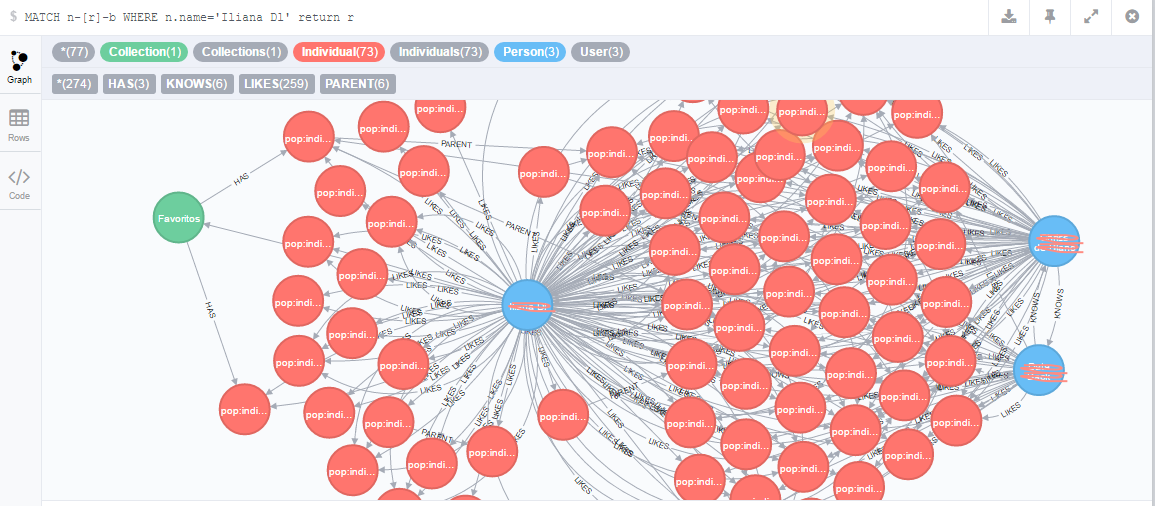
\includegraphics[width=3.5in]{img/gui-neo.png}
    \caption{Example query in Cypher.}
    \label{fig:cypher}
  \end{figure}

\item {\bf Relational Objects-PostgreSQL}
  The PostgreSQL relational database system is also employed because user 
  sessions and authentication,
  as well as dynamic web pages are handled directly by the Django web
  framework \cite{garcia2013evospace}. % these implementations details
                                % could go if needed. 

\item {\bf Interfaces}
The appropiate human interface will depend on the application domain, 
the current framework implemantation employs a web based application. Developers 
can use different templates, to present one or more phenotypes 
at a time, and the type of rating system: like or one to five stars. 
Another implementations do not need a graphical interface at all, for example the
EvoDraw instalation or the XYZ Project \cite{de2014artists}.   

\item {\bf Evolution}    
The evolutionary algorithm is decoupled from the data model, the algorithm 
could be implemented as an EvoWorker \cite{garcia2013evospace}, use an external library, 
or even assigned to humans. An additional tool was implemented for a human based evolution, 
where volunteers select the parents of the next generation and upload the 
new individuals \cite{de2014artists}.  
\end{itemize}

\section{Case Study: EvoDraw}
As a case study, a IEA was developed using the 
EvoSpace-Interactive (ES-I) platform \cite{garcia2013evospace}
A brief description of the application is presented next, focusing
on the data elements that where ported to the graph model.

\begin{figure}[!t]
    \centering
        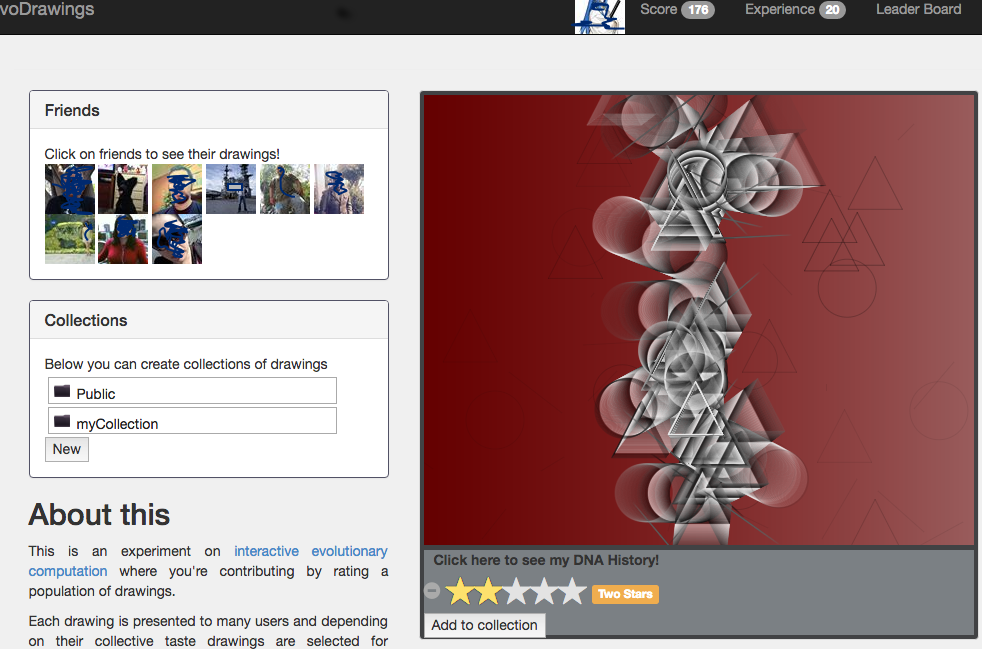
\includegraphics[width=3.5in]{img/interface.png}
    \caption{User interface of the EvoDrawings application.}
    \label{fig:web}
\end{figure}

\subsection{Fitness Assignment}
\label{sec:assignment}

The ES-I platform has been programmed to employ a 
collaborative methodology for performing fitness assignment. 
Several registered users assign a quality assessment to a single
phenotype and then an aggregated fitness value is calculated,
depending on the rating (from 1 to 5 stars) by each particular user,  
resulting in a many-to-many relationship between users and
phenotypes. Other components or users of the systems can 
query this user-phenotype relation to extract relevant
knowledge about the process and the population, for instance showing the
most popular phenotype, or the user with more participation 
\cite{picbreeder}.
In order to do this, metadata about phenotypes 
must be permanently stored, even
if they are no longer in the active population. 

\subsection{Collaboration}
\label{sec:col}
Users need to authenticate themselves to the system using their
Facebook account. In that sense, some users might not be interested
either because they do not want to give that information or simply because
they do not use that particular social network. Even as we might lose
some users that way, the additional information we obtain for scoring
phenotypes more than compensates for that. 
After entering the web application by using their Facebook account,
users can collaborate with their Facebook friends, 
sharing those phenotypes they like, or by taking phenotypes
from their friend's collections by using the web interface depicted 
in Figure \ref{fig:web}.
At the top left corner a list of Facebook friends is presented
to encourage users to interact with the system. In the central 
\emph{ Wall } area, a phenotype sampled from the population that is
being evolved via the evolutionary algorithm 
is shown to the user.
Here, the user can interact with the system in two ways.
First, he can assign a rating to the phenotype using
a five star rating system or,
additionally, a user can choose to add an image to one of their \emph{Collections}.
A collection is a special folder that stores those phenotypes a user likes and wishes
to save. After the user finishes interacting with the phenotype
on the Wall, he can choose to retrieve a new one from the population.
At the left hand side of Figure \ref{fig:web}, the web page shows the \emph{Collections} section.
The user can create several collections, to group and organize his favorite 
artifacts. Moreover, users can browse the content of each collection and from
there share images through their social network. This makes the assignment 
of fitness through the rating system a {\em social} activity, 
pursuing the objective of this work, which is to increase engagement of the users.

\subsection{Graph Model} 
The graph model for the EvoDraw applications has the following types of
nodes: {\bf User}, {\bf Phenotype} and {\bf Collection} . The Collection node represents
a collection of drawings belonging to users. One collection can contain many phenotypes 
or be empty. A single phenotype could be shared by many collections. The interaction 
between these entities are represented by the following edges:

\begin{itemize}
\item {\bf Likes} This relation describes the interaction between a user and
a phenotype in which a rating value is assigned.

\item {\bf Knows} The relation connects two users that know each
other in the Facebook social graph. 

\item {\bf Parent} Describes what phenotype is the parent of a new
  phenotype. 

\item {\bf Has} The relation describes an ownership relation between users and
those collections they own. 
\end{itemize}

\subsection{Gamification}
The rewarding mechanism as it is applied in EvoDraw gives more importance 
to the preference of those users with higher reputation
as given by their score points and experience levels.  
Each time a user does on of these actions their score is incremented by one:
\begin{itemize}
\item Start a session.
\item Rate a phenotype.
\item Create a collection.
\item Save a phenotype of the wall to a collection.
\item Save a phenotypes from a friend's collection.
\item Explore collections of other friends.
\end{itemize}

Two variables are used to determine the weight of a user's preference:
\begin{itemize}
\item {\em Experience}: This variable depends on the score and is a value 
between 0 and 100. It is assumed for this case, that once a user
reaches a 100 actions, it has enough experience on using the application.   

\item {\em Participation}: This variable is simply the degree of the user node 
in the graph.    
\end{itemize}

\subsection{Experimental Setup}
\label{sec:experiments}
 
Three versions of EvoDraw were compared:
\begin{itemize}
\item Base (B). All users have the same weight.
\item Non Graph Gamification (G). Only experience is considered
\item Graph Gamification (GG) . Both experience and participation are considered.
\end{itemize}
When gamification was employed, all score values known where presented to users
and a ranking of users by weight was shown in a window.
The three versions of the EvoDrawing web application were deployed to the
Heroku cloud service with the same configuration: Heroku Free option with a 512 MB of RAM, 
adding only the GrapheneDB and RedisTOGO plug-ins.

Table \ref{tab:params} shows the parameters used for the evolutionary algorithm. 

\begin{table}
  \small
  \caption{ Parameters for experiments.  }
  \label{tab:params} 
  \centering
  \small
  \begin{tabular}{l  c}
    \hline\noalign{\smallskip}
     Parameter & Value \\
    \noalign{\smallskip}\hline\noalign{\smallskip}
    Initial Population Size   & 80 \\ \hline
    Sample Size & 1 \\ \hline
    Step Size & 8 Samples \\ \hline
    Mutation &  \\ \hline
    Selection & Tournament \\ \hline
    Tournament Size &  6 \\ \hline
  \end{tabular}
\end{table}

% Anuncements
At the start of every experiment, a call to participation was issued
through social networks.  The link used in the call for participation
was shortened Google URL, that provides metadata and analytics for the
users that click on it.  In table \ref{tab:urls} the URL for each 
deployment in the Heroku platform is shown,
along with the short URL and the analytics link. In the same table a link to the GitHub 
application repository used to deploy to Heroku is also listed.    

Only data for the first week of deployment was considered 
for the experiments, and they where conducted 
between January and May of 2016. 

\subsection{Results} 
Before launch, each deployment was first tried with a few beta testers. 
When applying the leader board gamification technique for the first time a 
problem was found in this stage. The problem was that some users were cheating by giving a
rating to an animation even before it was returned from the server, this was done by just
constantly clicking the mouse button. This is a common problem found in systems using leader
boards because by making the scores visible to other players they are encouraged 
to compete \cite{hickman2010total}. The results of each of the three experiments in 
terms of participation are detailed next.

\begin{table}
  \small
  \caption{ After a week of the announcement the total number of volunteers, 
  nodes and edges in the graph and analytics URLs}
  \label{tab:urls} 
  \centering
  \small
  \begin{tabular}{l l l l l}
    \hline\noalign{\smallskip}
     Deployment &  Users &  Nodes &  Edges & URL \\
    \noalign{\smallskip}\hline\noalign{\smallskip}
    B   & 53 &  595   & 2220  & goo.gl/jLis4Q.info \\ \hline
    G   & 54 &  648   & 2596  & goo.gl/jqjNy5.info \\ \hline
    GG  & 68 &  932   & 3594  & goo.gl/J8TCe1.info \\ \hline
    \end{tabular}
\end{table}

Table \ref{tab:urls} shows the total number of volunteers, nodes and edges 
in the graph after each experiment. Moreover, the total number of evaluated 
phenotypes for each volunteer is presented in figure 
\ref{fig:top-ranked-participation} where users are ranked by the 
number of phenotypes they rated, in the \emph{x} axis is the rank, and in the \emph{y} axis 
the number of phenotypes evaluated using a logarithmic scale. Results show that when 
considering deployments B and G, the difference came with users with a medium level of participation.
When comparing all the experiments the deployment GG had the higher number of participation in users of all levels.    

\begin{figure}[!t]
    \centering
        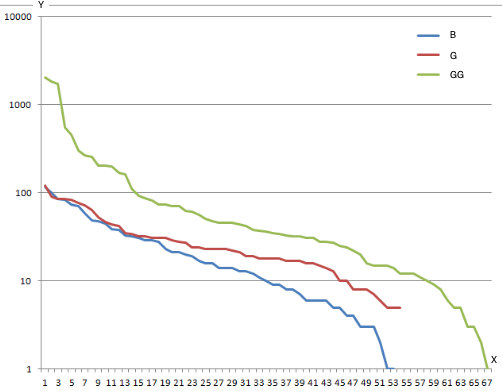
\includegraphics[width=3.3in]{img/comparison.png}
    \caption{Users ranked by the number of phenotypes they rated vs. the number of phenotypes evaluated using a logarithmic scale. }
    \label{fig:top-ranked-participation}
\end{figure}

Moreover, modeling the performance of an C-IEC system
involves understanding its dynamics. Previous works on browser-based
volunteer computing have used metrics basic such as: 
the number of users or the time spent by every one in the
computation \cite{DBLP:journals/gpem/LaredoBGVAGF14, 2016arXiv160101607M}. 
While works on other platforms such as SETI@home
\cite{javadi2009mining} have found that the Weibull, log-normal, and
Gamma distributions where viable modeles of the  
the availability of computing resources in several clusters.
This is in concordance with the results obtained in \cite{agajaj}, and also
browser-based volunteer evolutionary systems like NodIO \cite{DBLP:conf/gecco/MereloCGCRV16}.
The shape of those distributions is a skewed bell
with more resources in the {\em low} areas than in the high areas:
there are many users that give a small amount of cycles, while there
are just a few that give many cycles. 

In orther to assess if C-IEC follow the same pattern, even when
using gamification techniques, participation was fittted to a 
Weibull distribution, results in figure \ref{fig:w2} and figure \ref{fig:w3}
show that the same pattern appears in this case study. 


\begin{figure}[!t]
    \centering
        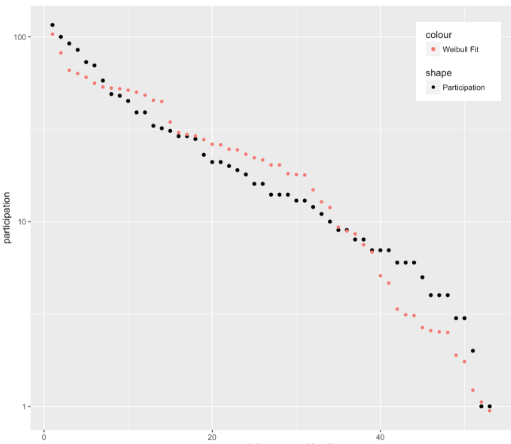
\includegraphics[width=3in]{img/weibull_2.png}
    \caption{Experiment 2. Weibull Fit}
    \label{fig:w2}
\end{figure}
\begin{figure}[!t]
    \centering
        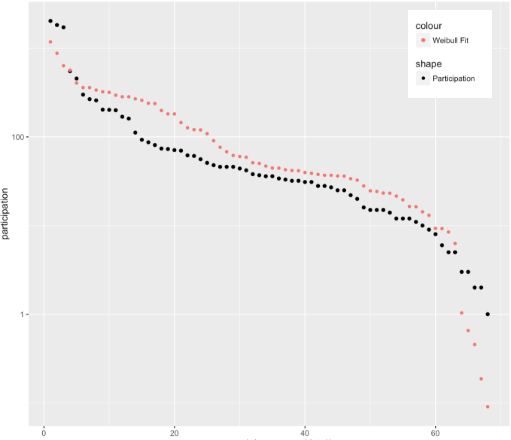
\includegraphics[width=3in]{img/weibull_3.png}
    \caption{Experiment 3. Weibull Fit}
    \label{fig:w3}
\end{figure}


\section{Case Study: EvoDraw-Kinect}

A variation of the previous application is The EvoDraw installation , using the same
framework but with a different form of interaction. Humans interact with the animations 
by simply looking at them. Again the population is stored in the EvoSpace container and
client computers remove animations from the EvoSpace to be presented in a display one at a time. 
After a certain amount of time,  animations are put back to the server along with information 
generated from the interaction. To continue, another is again removed and presented to viewers. 
An important feature is that once an animation is removed from the server, no other client can remove it, 
until the client that remove it puts the animation back, this means that any
animation is been shown only on one client at a given time. This cycle continues until there
is enough interactions to create a new generation of animations. 

In order to assign a fitness value to each animation and thus enabling the EA the selection of the more interesting animations, a natural user interface device (Kinect sensor for Xbox One)
is used for facial tracking. Each animation is 
presented several times in a single generation and the best are always passed to the next, 
with its fitness recomputed. To generate the new population the same operators as the previous case study
are applied to the population. 

\begin{figure}[!t]
    \centering
        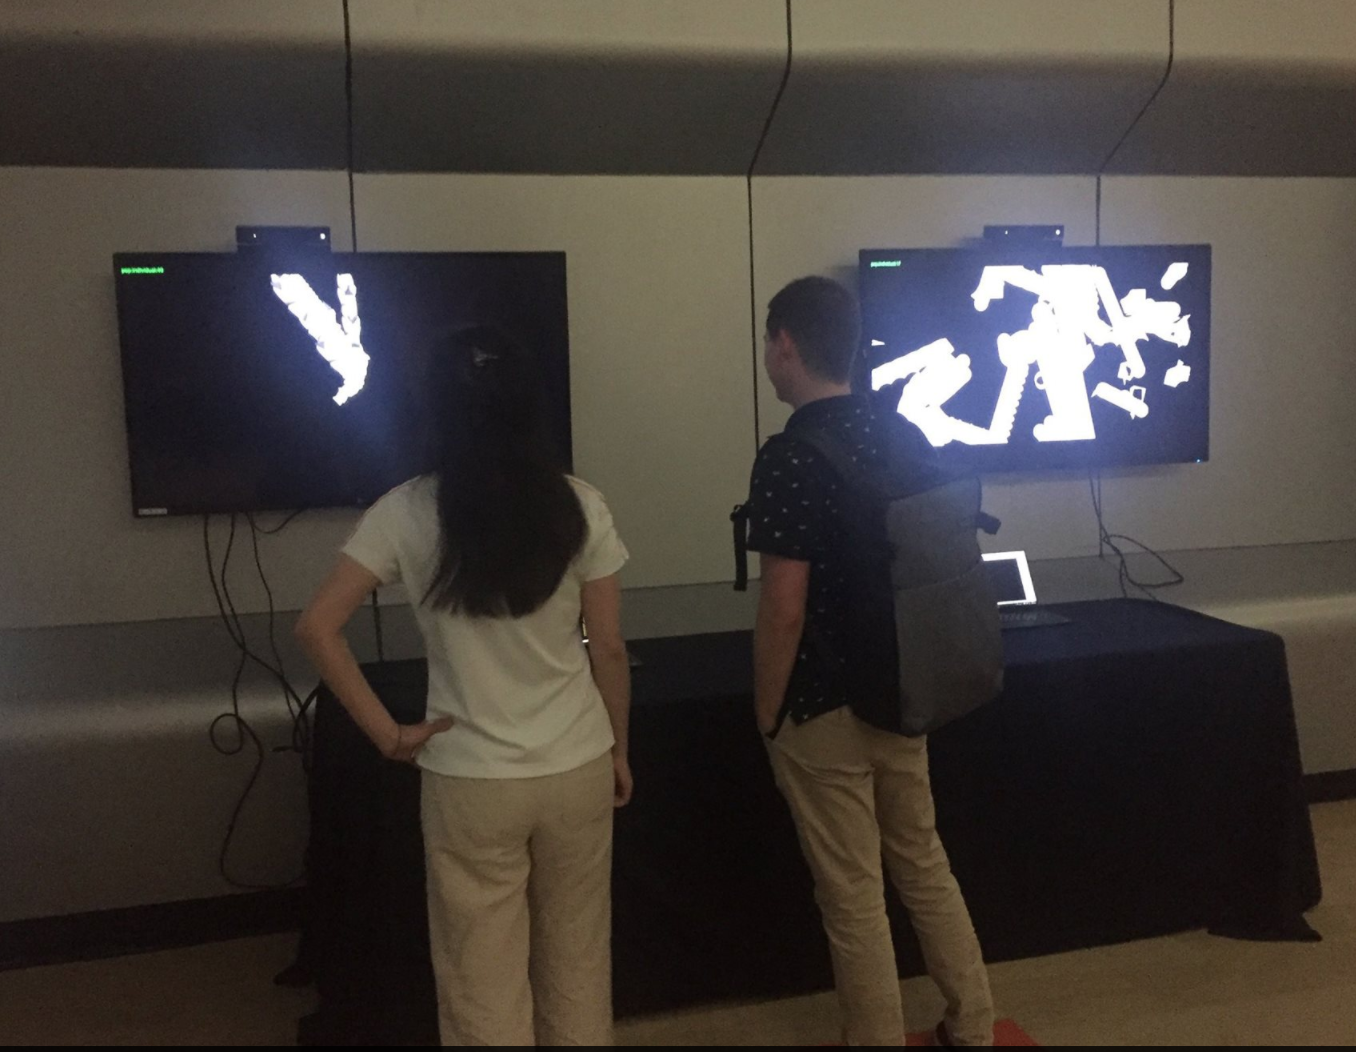
\includegraphics[width=3.5in]{img/kinect.png}
    \caption{EvoDraw Instalation on Alife XV Cancun Mexico.}
    \label{fig:kinect}
\end{figure}

In this instalation the components of the framework used where the EvoSpace and the Evolutionary Algorithm.
Information from users was limited to a stream of readings from the sensor.

\section{Case Study: XYZ-Unplugged}

XYZ is a collective artwork generated by means of the Unplugged version of the Evolutionary Algorithm.
While in the previous cases software tools are in charge of running the EA and users collaborate evaluating
fitness quality, the sframework in XYZ is only in charge of storing digital versions of the works produced 
by the team of artists, who are really in charge of applying every step of the evolutionary algorithm. In 
this case only the relations are stored, and a basic user profile. 

Thus, the main difference between the standard IEC and the Unplugged EA, is that in the latest,
every genetic operation as well as the general evolutionary loop is in charge of human beings. 
Thus the team of artists are in charge of:  (i) setting up the initial population by selecting
well known works from the history of arts;  (ii) each of the artists selects every generation two works 
from the previous one, and produce a new painting by applying any kind of crossover and mutation he may consider 
(iii) the process repeats for the number of generations initially decided, so that at the end, a collective 
artwork has been produced including as many paintings per generation, as artists are participating in the experiment.  

Artists resort to framework as the tool allowing them to store the paintings, deciding their preferred ones from the
previous generation, as well as describing the reasons for their selections, mutation and crossover operations applied.
The tool is also in charge of generating statistics, computing \textit{elitism}, thus adding the most selected work to 
the next generation, etc.

\begin{figure}[!t]
    \centering
        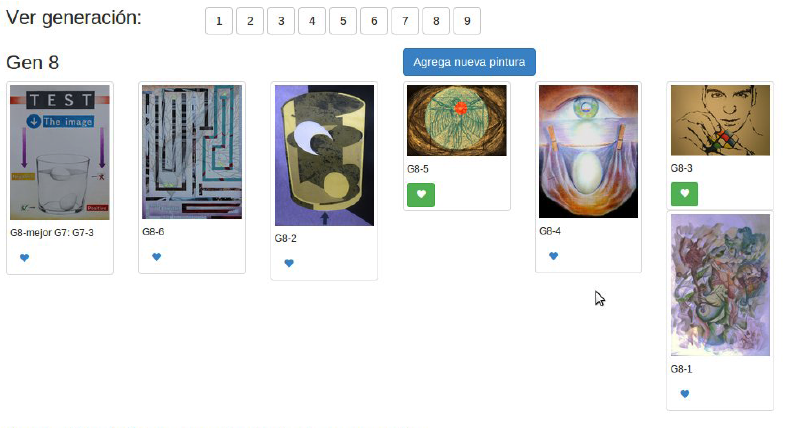
\includegraphics[width=3.5in]{img/interfaceXYZ.png}
    \caption{User interface of the XYZ application.}
    \label{fig:xyz}
\end{figure}

\section{Conclusions}
\label{sec:conclusions}

Collaborative and volunteer based IEC systems involve the dynamic 
interaction of many entities and artifacts. Employing human centered approach 
can benefit researchers to understand and visualize this kind of systems better.
In this paper a human-centered software framework was proposed, and was validated
through the implementaion and refinement of three C-IEC applications.
This framework enabled the implementation of a gamification technique 
to improve engagement in a case study. Providing a common arena where users are aware of the
activities of other users in the social vicinity. Following a hybrid data model approach
gives developers and project owners options when innovating with other means
of interaction or new applications.

One of the interesting future lines of work would be to look a bit
more closely at the behavior of users as they are rating artifacts 
in the web system. These initial experiments hint at a possible power law, which might indicate that
the IEC system could be self-organizing, a process that would allow it
to reach a critical state, as has been found in software repositories,
for instance \cite{Merelo2016:repomining}. 
The dynamics of this kind of system are fundamentally different, and our future research will
include exploring these aspects of the system. 

Another line of work would be to study the negative effects of using 
gamification techniques to improve engagement, like cheating or competition.
Finally, the refinement of the proposed Human-Centered framework will need
more case studies and further multi-disciplinary research. 



\begin{acks}
  % The authors would like to thank Dr. Yuhua Li for providing the
  % matlab code of  the \textit{BEPS} method. 

  % The authors would also like to thank the anonymous referees for
  % their valuable comments and helpful suggestions. The work is
  % supported by the \grantsponsor{GS501100001809}{National Natural
  %   Science Foundation of
  %   China}{http://dx.doi.org/10.13039/501100001809} under Grant
  % No.:~\grantnum{GS501100001809}{61273304}
  % and~\grantnum[http://www.nnsf.cn/youngscientsts]{GS501100001809}{Young
  % Scientsts' Support Program}.
  Reserved\\
  Space\\
  for\\
  Acks

\end{acks}


\bibliographystyle{ACM-Reference-Format}
\bibliography{sigproc,../bib/biblio,../bib/evospace-i,../bib/volunteer,geneura} 

\end{document}
